\documentclass[../../../../document.tex]{subfiles}

\begin{document}
    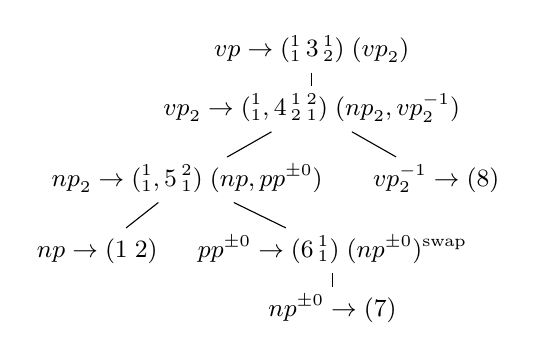
\begin{tikzpicture}[
        level distance=7mm,
        font=\small,
        sibling distance=10mm,
        anchor=center,
        every node/.style={text height=2.5mm},
        rounded corners=0,
        baseline=(mid.base)
        ]
        \begin{scope}[level distance=7.5mm]
            \node (troot) {\(\cn{vp} \to (\x^1_1\,3\,\x^1_2)\;(\cn{vp}_2)\)}
            child {node {\(\cn{vp}_2 \to (\x^1_1, 4\,\x^1_2\,\x^2_1)\;(\cn{np}_2, \cn{vp\binsym}_2^{-1})\)}
                [sibling distance=9em, level distance=9mm]
                child {node (mid) {\(\cn{np}_2 \to (\x_1^1, 5\,\x^2_1)\;(\cn{np}, \cn{pp}^{\pm 0})\)}
                    [sibling distance=8.5em]
                    child {node[xshift=1em] {\(\cn{np} \to (1\;2)\)}}
                    child {node[xshift=1em] {\(\cn{pp}^{\pm 0} \to (6\,\x^1_1)\;(\cn{np}^{\pm 0})^{\mathrm{swap}}\)}
                        [level distance=7.5mm]
                        child {node {\(\cn{np}^{\pm 0} \to (7)\)}}}}
                child {node {\(\cn{vp\binsym}_2^{-1} \to (8)\)}}};
        \end{scope}
    \end{tikzpicture}
\end{document}